This chapter contains the background knowledge to optimise the understanding of patellofemoral pain and deep learning. The chapter is divided into the following sections: Anatomy of the knee, Pain, Pain mapping and Knee regions. Futhermore, machine learning and deep learning are specified.


\section{Anatomy of the Knee}
The knee is the largest synovial joint in the body and consists of a hinge and a gliding joint. The hinge joint is placed between the lateral and medial femoral condyles and the lateral and medial tibial condyles. The gliding joint is formed between the patella and femur. The structure of the knee is illustrated in figure \ref{fig:bonestruc}.\citep{Martini2012}

\begin{figure} [H]
\centering
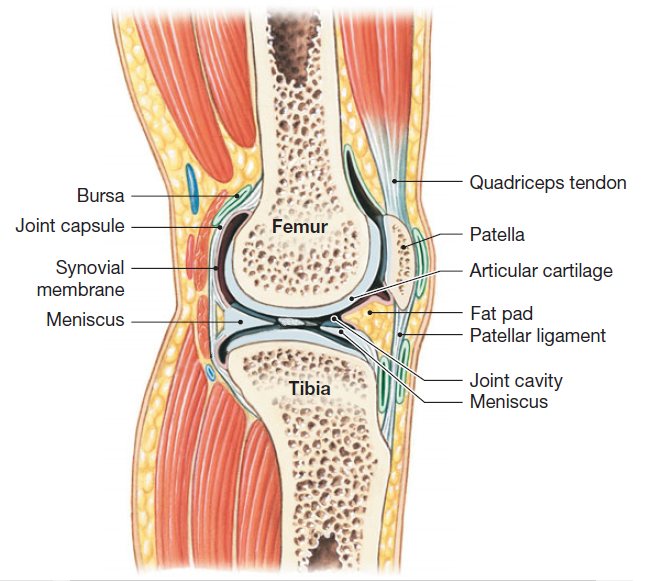
\includegraphics[width=0.7\textwidth]{figures/bonestruc}
\caption{The figure illustrates the anatomy of the knee. Edited from \citep{Martini2012}.}
\label{fig:bonestruc}
\end{figure}

\noindent
It is shown in figure \ref{fig:bonestruc} that the patella is a sesamoid bone. At birth the patella consists of cartilaginous and ossifies when the child’s extremities gets stronger, which typically proceeds between age two or three and the beginning of puberty. \\
\noindent
The patella is surrounded by the tendon of the quadriceps femoris. Quadriceps femoris is the muscles which controls the extending of the knee. The quadriceps tendon is combined to the surface anterior and superior of patella. Tibia is combined to the anterior and inferior surface of the patella by the patellar ligament. The bones, tibia and femur, are covered by articular cartilage with the purpose of protecting the bones from friction. The articular cartilage on the two bones are separated from one another by synovial membranes that contains synovial fluid, that further reduce the friction. The primary functions of the synovial fluid is to lubricate, distribution of nutrient and absorption of shock.\citep{Martini2012}

The fat pads and menisci are placed between the articular cartilages. The fat pads’ function is to protect the cartilage and fill out space as result of the joint cavity changes. The menisci stabilize the knee and acts like pads, that conform shape when femur moves. In addition to fat pads and menisci the bursa acts as friction minimization between patella and tissues.\citep{Martini2012} \\
There are three separate articulations in the knee joint. The first is between the patella and the patellar surface of the femur and the rest are between the femoral and tibial condyles. Additionally, the knee consist of seven major ligaments that stabilize the knee joint, which is shown in figure \ref{fig:knee}.\citep{Martini2012}

\begin{figure} [H]
\centering
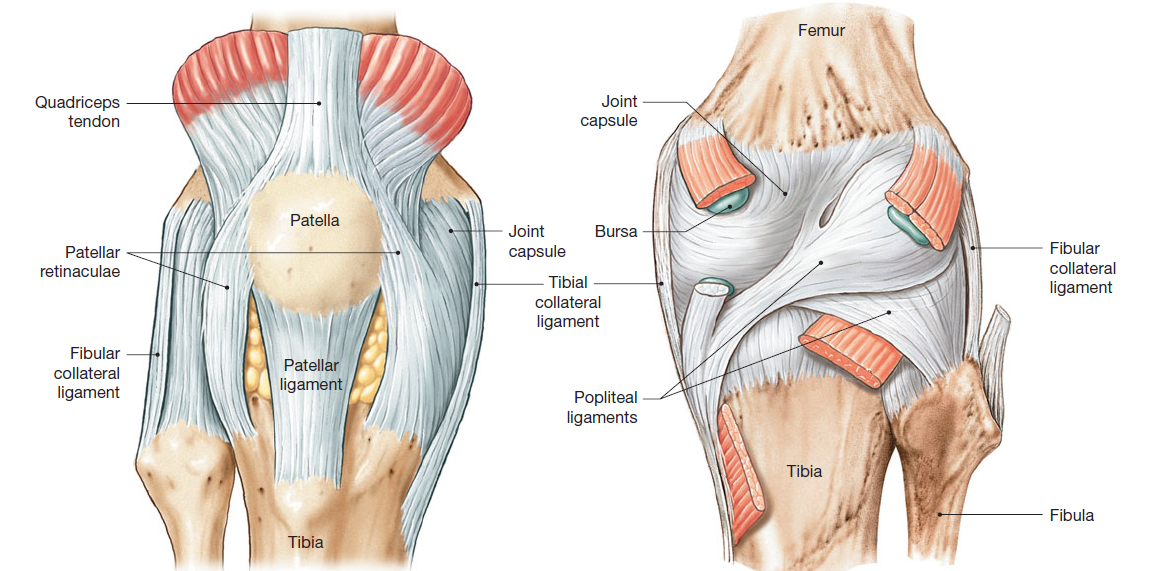
\includegraphics[width=1\textwidth]{figures/knee}
\caption{The figure illustrates the anatomy of the knee with focus on the ligaments. Edited from \citep{Martini2012}.}
\label{fig:knee}
\end{figure}

\noindent
The ligaments patellar retinaculae and patellar ligament support the anterior surface of the knee. When the knee is fully extended, the tibial and fibular collateral ligament are responsible for stabilizing the joint. Between femur and the two lower bones in the leg, tibia and fibula, is the location of the two popliteal ligaments, which stabilize the posterior surface of the joint. In addition to the visible ligaments in figure \ref{fig:knee} there are the anterior cruciate ligament (ACI) and posterior cruciate ligament (PCI) in the joint capsule. The two ligaments cross each other and are connected to the tibial and femoral condyles. They reduce the movement, anterior and posterior.\citep{Martini2012}

As previously mentioned the gliding joint is formed between the patella and femur, so that during knee movement patella is gliding up and down at the femoral condyle. A condition associated with incorrect movement of the patella, is patellofemoral pain syndrome (PFPS), that occurs when the patella moves outside of its ordinary track, which for instance can be movement in lateral direction.\citep{Martini2012}


\section{Pain}
Pain is experienced and perceived subjectively and there is a lack of methods to measure pain accurately \citep{IASP2012, Younger2009}. 
The International Association for the Study of Pain (IASP) has defined pain as being “an unpleasant sensory and emotional experience associated with actual or potential tissue damage” \citep{IASP2012}.

Physiologically pain can be divided into three categories: acute pain (less than three months), persistent or chronic pain and cancer pain. Furthermore, pain can be either nociceptive or neuropathic. Nociceptive pain is associated with tissue damage. Neuropathic is associated with damage to the nervous system.\citep{Briggs2010} 

There are many ways of measuring pain, but none of them are an valid or reliable in terms of objectively quantifying a subjects experienced pain \citep{Younger2009}. One the methods used to meassure pain is called pain maps which is where the subject draws their precived pain onto an illustration of the human body. This method will be discriped further in the following section.   


%OOOOOOOO TRANSITION TO PAIN MAPPING OOOOOOOOOOOOOO (it's hard to describe pain and so on...)

\subsection{Pain mapping}
Pain mapping is a technique, that Harold Palmer introduced in 1949 \citep{Grunnesjo2006}, which is used to transfer a patient’s perceived pain into an objective graph or map by drawing the pain area. Pain drawings can be made by the patients who draw their pain areas on a display on which a body outline is shown, or it can be made by observers who observe the patients and then draw from the signs the patients are showing. An example of a body outline is shown at figure \ref{fig:painmap}. Sometimes a questionnaire is added to the pain drawings to get a more detailed overview of the pain.\citep{Schott2010}

\begin{figure} [H]
\centering
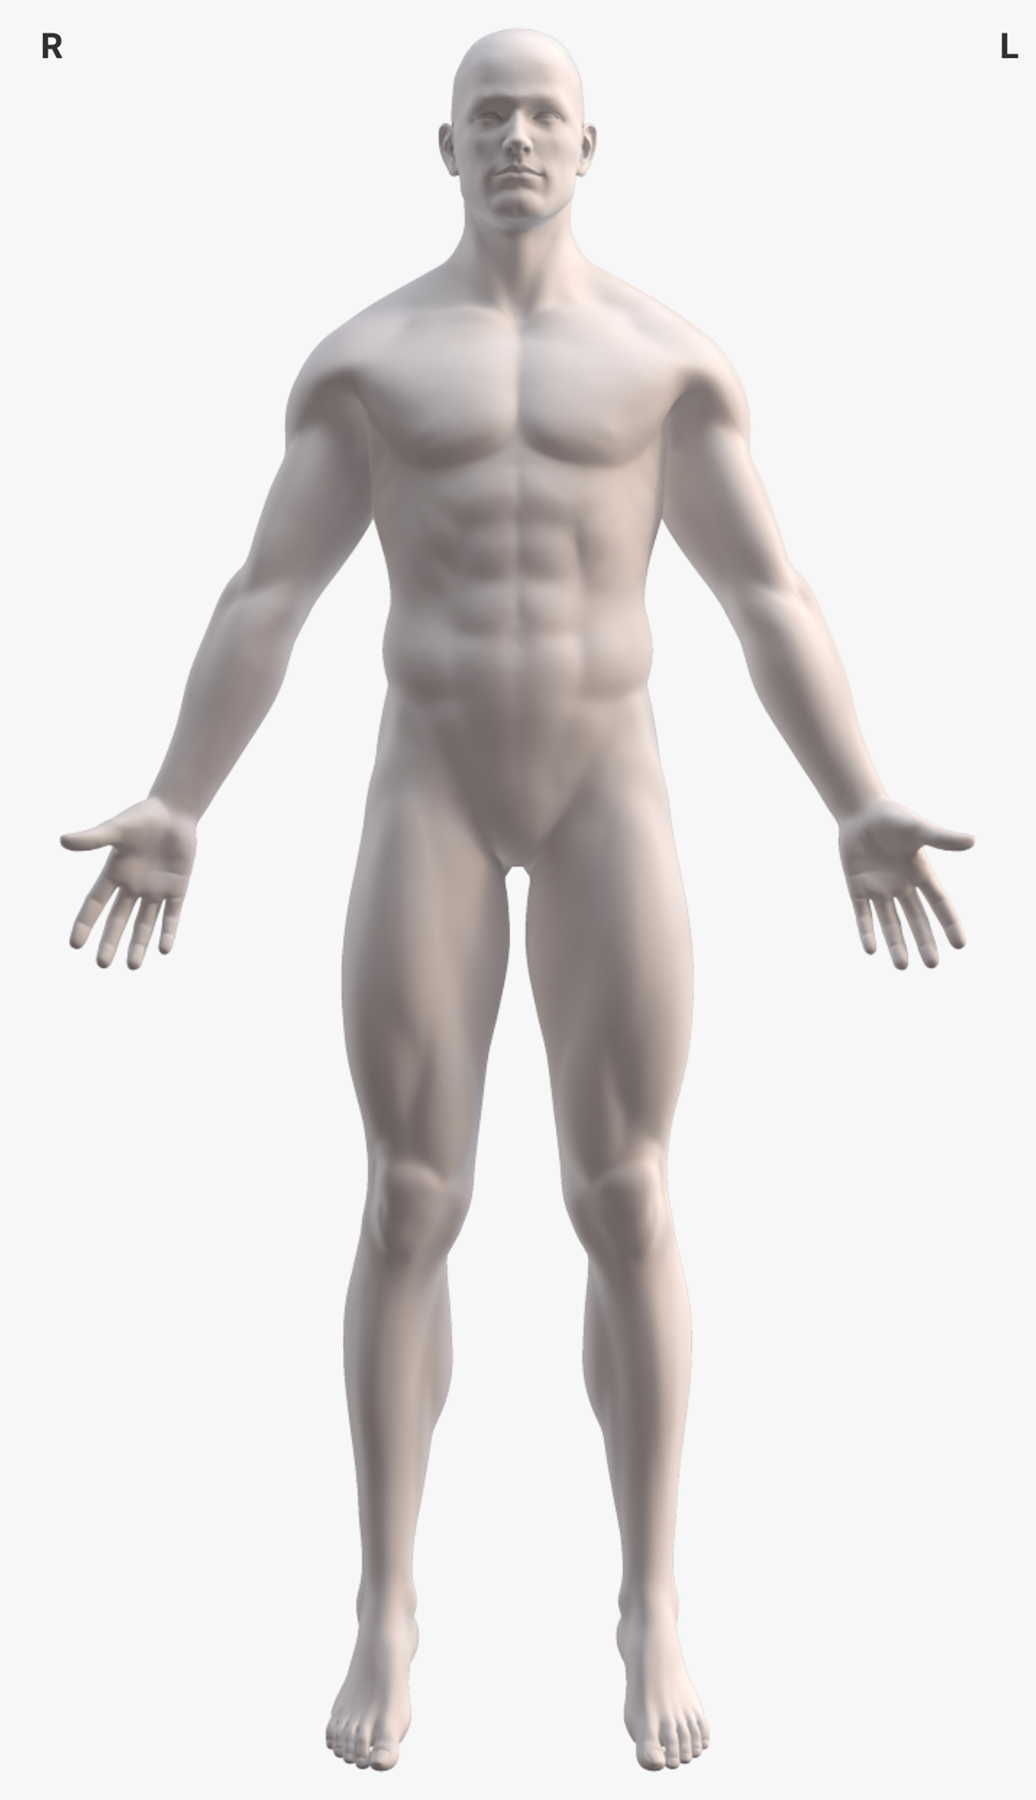
\includegraphics[width=0.4\textwidth]{figures/painmap}
\caption{The figure illustrates an anterior body outline for pain drawing. The figure is a screenshot from the application Navigate Pain.}
\label{fig:painmap}
\end{figure}

Pain mapping are commonly used in clinical practice \citep{Schott2010}, and can be useful for patients when they try to describe their pain. Pain maps may also be helpful in diagnosing patients and follow-ups during or after treatment to get an indicator of the patient’s response to the treatment.\citep{Boudreau2016}
According to \citeauthor{Schott2010} there are some issues with the graphical representations of pain, some of which are problems with drawing a three-dimensional feeling of pain on a two-dimensional surface, and distinguishing between internal and external perceived pain on a map.\citep{Schott2010}

\section{Knee regions}
Patients with PFP often describe the knee pain as a diffuse pain, and when looking at pain drawing samples from multiple patients it is also evident that there is a high variability in the distribution of pain patterns across different areas of the knee. 
To distinguish between different pain areas, the knee can be divided into various regions as seen in figure \ref{fig:atlas}, where atlases of the left and right anterior knees are illustrated. The atlases has been provided by Shellie Boudreau. 

\begin{figure} [H]
\centering
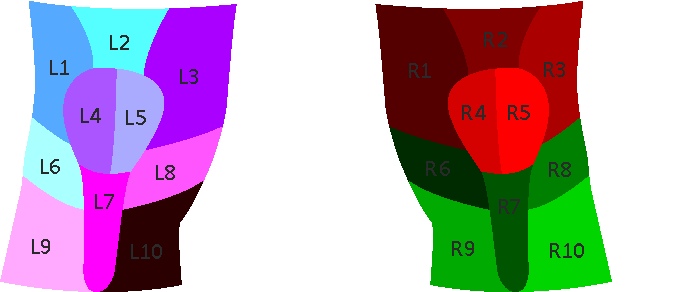
\includegraphics[width=0.6\textwidth]{figures/atlas}
\caption{The figure illustrates atlases of the left and right knees, where each knee is split into ten regions.}
\label{fig:atlas}
\end{figure}

\newpage